

%\newcommand*{\ACM}{}%

\ifdefined\ACM

%\documentclass[sigplan,screen]{acmart}
  \documentclass[manuscript,screen,review]{acmart}

\else
  \documentclass{article}
  \usepackage[utf8]{inputenc}
\usepackage[a4paper, total={6in, 9in}]{geometry}
\usepackage{braket}
\usepackage{xcolor}
\usepackage{amsmath}
\usepackage{amsfonts}
\usepackage{amsthm}
\usepackage{amssymb}
%\usepackage[ocgcolorlinks]{hyperref}
\usepackage{hyperref}
%\usepackage{hyperref,xcolor}
%\usepackage[ocgcolorlinks]{ocgx2}
\usepackage{cleveref}
\usepackage{graphicx}
\usepackage{svg}
\usepackage{float}
\usepackage{tikz}
\usetikzlibrary{patterns, shapes.arrows}
\usepackage{adjustbox}
%\usepackage{tikz-network}
\usepackage{tkz-graph}
\usepackage{tkz-berge}
\usepackage[linesnumbered]{algorithm2e}
\usepackage{multicol}
\usepackage[backend=biber,style=alphabetic,sorting=ynt]{biblatex}
%\usepackage{xcolor}
%\usepackage{tkz-berge}
%\usepackage{tkz-graph}
\usepackage{pgfplots}
\usepackage{sagetex}
\usepackage{setspace}
\usepackage{etoc}
%\usepackage{wrapfig}
\usepackage{pgfgantt}
\DeclareUnicodeCharacter{2212}{−}
\usepgfplotslibrary{groupplots,dateplot}
\pgfplotsset{compat=newest}

\newtheorem{theorem}{Theorem}
\newtheorem{definition}{Definition}
\newtheorem{example}{Example}
\newtheorem{claim}{Claim}
\newtheorem{fact}{Fact}
\newtheorem{remark}{Remark}
\newtheorem*{theorem*}{Theorem}
\newtheorem{lemma}{Lemma}
\crefname{lemma}{Lemma}{Lemmas}
\hypersetup{colorlinks=true}
% , allcolors=blue,allbordercolors=blue,pdfborderstyle={0 0 1}}
%\hypersetup{pdfborder={2 2 2}}
% pdfpagemode=FullScreen,
% backref 

\newtheorem{problem}{Problem}
\crefname{problem}{Problem}{Problems}

\DeclareMathOperator{\Ima}{Im}


  \addbibresource{./sample.bib} 

\fi

\begin{document}
\newcommand{\commentt}[1]{\textcolor{blue}{ \textbf{[COMMENT]} #1}}
\newcommand{\ctt}[1]{\commentt{#1}}
\newcommand{\prb}[1]{ \mathbf{Pr} \left[ #1 \right]}
\newcommand{\prbm}[2]{ \mathbf{Pr}_{ #2 }\left[ #1 \right]}
\newcommand{\prbc}[3]{ \mathbf{Pr}_{ #2 }\left[ #1 \right | #3]}
\newcommand{\prbcprb}[3]{ \prbc{#2}{#1}{#3} \cdot \prb{#3} } 
\newcommand{\expp}[1]{ \mathbf{E} \left[ {#1} \right]}
\newcommand{\onotation}[1]{\(\mathcal{O} \left( {#1}  \right) \)}
\newcommand{\ona}[1]{\onotation{#1}}
\newcommand{\PSI}{{\ket{\psi}}}
\newcommand{\xij} { X_{ij} } 
\DeclareMathOperator{\Ima}{Im}
%\newcommand{\LESn}{\ket{\psi_n}}
%\newcommand{\LESa}{\ket{\phi_n}}
%\newcommand{\LESs}{\frac{1}{\sqrt{n}}\sum_{i}{\ket{\left(0^{i}10^{n-i}\right)^{n}}}}
%\newcommand{\Hn}{\mathcal{H}_{n}}
%\newcommand{\Ep}{\frac{1}{\sqrt{2^n}}\sum^{2^n}_{x}{ \ket{xx}}}
%\newcommand{\HON}{\ket{\psi_{\text{honest}}}}
%\newcommand{\Lemma}{\paragraph{Lemma.}}
\newcommand{\Cpa}{[n, \rho n, \delta n]}
%\setlength{\columnsep}{0.6cm}
\newcommand{\Jvv}{ \bar{J_{v}} } 
\newcommand{\Cvv}{ \tilde{C_{v}} } 

\newcommand{\Gz}{ G_{z}^{\delta} } 
\newcommand{ \Tann } {  \mathcal{T}\left( G, C_0 \right) }
\newcommand{\ireducable}{ireducable \hyperref[ire]{[\ref{ire}]} }
\newcommand{\cutUU}{E(U_{-1} \bigcup U_{+1} ,U)} 
\newcommand{\wcutUU}{w\left( E(U_{-1} \bigcup U_{+1} ,U)  \right)}
\newcommand{\testgo}{  \mathcal{T}\left(J, q , C_{0}\right) } 

\newcommand{\duC}{\left( C_{A}^{\perp}\otimes C_{B}^{\perp} \right)^{\perp}}
\newcommand{\duduC}{\left( C_{A}\otimes C_{B}\right)^{\perp}}
  




\title{Magic States Distillation Using Quantum Expander Codes. } 
\author{David Ponarovsky}
\maketitle




%\begin{abstract}
%  We studies the complexity of synthesis quantum states using PRS, our reasch continues the work by \cite{searchtodecision}, \cite{rosenthal2023efficient}, \cite{rosenthal2021interactive}, \cite{metger2023stateqip}, \cite{delavenne2023quantum}.
%\end{abstract}
%
%

\begin{claim}
  Let $\Lambda$ be a set of independent $k^{\prime}$ codwords in $[n,k,d]$ code. Then there is a code $C^{\prime} = [\le 2n, \ge k-k^{\prime}/2, d]$and $\Lambda^{\prime}$ set of independent codewords of it, such that $|\Lambda^{\prime}| > \frac{1}{2}|\Lambda|$ and for every pair $x,y \in \Lambda^{\prime}$ we have that $x\cdot y = 0$.
\end{claim}
\begin{proof} 
  First, consider the trigonal/staris/square matrix given by gauss applying elimination on $\Lambda$. Now, consider the following process, go up hil in the squares matrix. Let $j$ be the first nonzero cordinate in the most down row in the matrix. In the $i$th iteration, we ask how many vectors $u_{m}$ such that $m < k^{\prime}-i$ are statisfies $u_{m} u_{k^{\prime}-i} = 0$. Now, if encoding the $j-i$ cordinate by $C_{0}^{1}$ such $1_{C_{0}^{1}}$ give $|B_{i} | > |\bar{B_{i}}|$ then choose to encode with $C_{0}^{1}$ otherwise encode that coordiante with $C_{0}^{0}$. 
\end{proof}

\newcommand{\hashcode}{ checks-hashed }

\ctt{Change to $ \prbm{ i,j \text{ collide  }  }{  j \sim [\Delta] } < \frac{1}{2\Delta}$ }


\begin{definition}
  Let $\{h_{i} \}_{1}^{t}$ be the checks of $\Delta$-length code $C_{0}$. We say that $i$th bit and the $j$th bit collide if there a check $h$ such that $h_{i}=h_{j}=1$. We say that a $C_{0}$ is a \hashcode if:  
  \begin{equation*}
    \begin{split}
      \prbm{ i,j \text{ collide  }  }{ i, j \sim [\Delta]^{2} } < \frac{1}{2\Delta}
    \end{split}
  \end{equation*}
\end{definition}

\begin{claim}
  Suppose that $C_{0}^{\perp}$ is a \hashcode. Then $\left( C_{0}^{\otimes m} \right)^{\perp}$ is also a \hashcode. 
\end{claim}
\begin{proof}
  
  \begin{equation*}
    \begin{split}
      \prbm{X^{(m)}_{u,v}}{u,v\sim [n]^{2}} \le & \prbm{X^{(1)}_{u,v}}{u,v\sim [\Delta]^{2}} \cdot \prbm{X^{(m-1)}_{u,v} }{u,v\sim [n/\Delta]^{2}} \\ 
      \le & \frac{1}{2\Delta} \cdot \left( \frac{1}{2\Delta} \right)^{m-1} = \left( \frac{1}{2\Delta} \right)^{m}
    \end{split}
  \end{equation*}
\end{proof}

Consider the following decoder, we flip a bit if flipping it decrease the syndrome. Now observers that if a non faulty bit $i$ has been flip then it means that there is at least one faulty bit $j$ in the error $e$ that $i,j$ collide. Similarly if a faulty bit $i$ hasn't been flip then it means that there is another faulty bit $j$ that collide with him. In overall we conclude that the total number of incorrect flips made by the decoder is at most the number of collisions. 

\begin{equation*}
  \begin{split}
    \expp{\sum_{v \in e} \sum_{u \in [n]} X_{v,u}} \le |e|\cdot n \cdot \left( \frac{1}{2\Delta} \right)^{m} = \frac{|e|}{2^{m}}
  \end{split}
\end{equation*}

Now we are going to add a random error at weight $\frac{|e|}{2^{m}}$ to ensure that in the next iteration the $\frac{|e|}{2^{m-1}}$ error will distributed uniformly. Repeating for $\log_{2^{m-1}}$ rounds correct the error. (not exactly there is an error in each round that should be handled).   

\ctt{ We flip in over all $|e| \sum \frac{1}{2^{i}}  < 2|e| $ bits, so we would like to have $|e| \le d/4 $.} 


\ctt{ Yet we can do better, if $ e = z + \tilde{e}$ where $z$ commute with all our generators. }

\ctt{ And if it anticommute with only $l$ of them, then we have only $l$ errors. }


\begin{equation*}
  \begin{split}
    \Delta^{m}\le 1/p^{2}_{0} & \rightarrow \alpha \cdot 1/p^{2}_{0} , \frac{m}{2^{m}} \log \Delta 
  \end{split}
\end{equation*}


\begin{claim}
Let $H$ be a $|V|\times r$ binary parity check matrix of $\tilde{C}$. Also, let $G$ be a $\Delta$-regular graph. A bit assignment over $G$ edges $x$ will be said to be $\tilde{C}$-vertices-respect if the vector $z(x) \in \mathbb{F}_{2}^{|V|}$ which is defined as:
  \begin{equation*}
    z(x)_{v} = \begin{cases}
      1 & v \text{ sees at least one } 1\\
      0 & \text{otherwise}
    \end{cases}
  \end{equation*}
   is a codeword of $\tilde{C}$. Let $\Lambda$ be the set of all $\tilde{C}$-vertices-respect assignments. Then $|\Lambda| > (1-\varepsilon)2^{\rho |V|}$.
\end{claim}

\begin{proof} 
Any $x \in \Lambda$ is a solution for the following system of equations:
  \begin{equation*}
    \begin{split}
      z_{v} &= 1 + \prod_{ e \in v }{ \left( 1 - x_{e} \right) } \\
      Hz &= 0
    \end{split}
  \end{equation*}
\end{proof}

\begin{claim}
  Assume that $C_{0}$ is a $\Delta$-length code such that for any two non-trival codewords $c,c^{\prime}\in C_{0}$ we have that $c\cdot c^{\prime}=1$, and denote by $C = \mathcal{T}(G,C_{0})$. And let $\Lambda$ be a the set of all $\tilde{C}$-vertices-respect assignments where $\tilde{C}$ satisfies relation $R$. Then also $C \cap \Lambda$ satisfies $R$. 
\end{claim}





Let $\ket{f}$ be a codeword in $C_{X}$, and let $X_{g}$ be the indicator that equals $1$ if $f$ has support on $X_{g}$, and $0$ otherwise. Observes that applying $T^{\otimes}$ on $\ket{f}$ yilds the state: 
\begin{equation*}
  \begin{split}
    T^{\otimes n}\ket{f} & =  T^{\otimes n}\ket{\sum_{g} X_{g}g } = \exp \Big( i\pi/4 \sum_{g} X_{g}|g|  -  2 \cdot i \pi/4 \sum_{g,h} X_{g}X_{h}|g\cdot h| \\
    & +  4 \cdot i\pi/4 \sum_{g,h} X_{g}X_{h}X_{l}|g\cdot h \cdot l| -   8  \cdot i\pi/4 \cdot \text{ integers } \Big) \ket{f} \\
    & = \exp \Big( i\pi/4 \sum_{g} X_{g}|g|  -  2 \cdot \pi/4 \sum_{g,h} X_{g}X_{h}|g\cdot h| +  4 \cdot i\pi/4 \sum_{g,h} X_{g}X_{h}X_{l}|g\cdot h \cdot l| \Big) \ket{f}
  \end{split}
\end{equation*}

\section{Many to One.}
Assume that $f$ is supported on exactly one generator. Then we have that $T^{\otimes n}\ket{f}  = e^{i\pi|g|/4}\ket{f}$ Therefore, if $|g| = 4k+1$ then we are done.


\section{Using Quntum Error Correction Codes.}

Now assume that the code $C_{X}$ is the quantum Tanner code, denote by $G,A,B$ the group and the two generator sets that are used for constructing the square complex. 

\begin{claim} 
Consider $g,h$ that are supported on the same $v\in V$. We will call such a pair a source-sharing pair. Suppose that for any we have that $|g \cdot h|$ is even. Then there is a Clifford gate that computes $\ket{f} \mapsto \exp \Big(  -  i\pi \sum_{g,h \text{ source-sharing }} X_{g}X_{h}|g\cdot h|  \Big) \ket{f} $.
\end{claim}
%
%%\begin{claim}
%%  \label{claim:phase}
%%  The gate $\ket{f} \mapsto \exp \Big(   i\pi \sum_{g,h} X_{g}X_{h}X_{l}|g\cdot h \cdot l| \Big) \ket{f} $ is in the Clifford group.  
%%\end{claim}
%%
%%\begin{proof}
%%  Just decode $f$ and apply \textbf{CCZ} between any triple of qubits corresponding to the generators $g,h,l$ such that $g \cdot h \cdot l=_{2} 1$. Then encode the state again. Observes that \textbf{CCZ} is a Clifford gate, and by the fact that the code is a CSS code then the decoder and the encoder are both in the Clifford.
%%\end{proof}
%%
%
%
%\section{Fail Attempt.}
%
%
%In addition, let us assume the existence of $d \in G$ such that $d$ is non-identity and commutes with any element in $A \cup B$. Then, observe that multiplying by $d$ preserves adjacency on the complex. Namely, if $\{u,v\} \in E$ then also $\{du, dv\} \in E$. 
%
%Consider $\ket{f}$ such that if $X_g$ is not zero, and $g$ is associated with a local codeword $c \in C_A \otimes C_B$ on vertex $v$, then the generator associated with the local codeword $c$ on vertex $d \cdot v$ also supports $f$, denoted by $g'$. Thus, the exponent above becomes:
%
%\begin{equation*}
%  \begin{split}
%    & = \exp \Big( i\pi/4 \sum_{g} X_{g}|g|  -  2 \cdot \pi/4 \sum_{g,h \in G /a} X_{g}X_{h}|g\cdot h| + X_{g^{\prime}}X_{h^{\prime}}|g\cdot h |  \\
%    & +  4 \cdot i\pi/4 \sum_{g,h \in G/a} X_{g}X_{h}X_{l}|g\cdot h \cdot l| + X_{g^{\prime}}X_{h^{\prime}}X_{l^{\prime}}|g\cdot h \cdot l| \Big) \ket{f} \\
%    & = \exp \Big( i\pi/4 \sum_{g} X_{g}|g|  -  2 \cdot 2 \cdot \pi/4 \sum_{g,h \in G/a} X_{g}X_{h}|g\cdot h| +  2 \cdot 4 \cdot i\pi/4 \sum_{g,h \in G/a} X_{g}X_{h}X_{l}|g\cdot h \cdot l| \Big) \ket{f} \\
%    & = \exp \Big( i\pi/4 \sum_{g} X_{g}|g|  -  i\pi \sum_{g,h \in G/a} X_{g}X_{h}|g\cdot h|  \Big) \ket{f} 
%  \end{split}
%\end{equation*}
%
%\begin{figure}
%  \centering
%  \scalebox{0.1}{
%    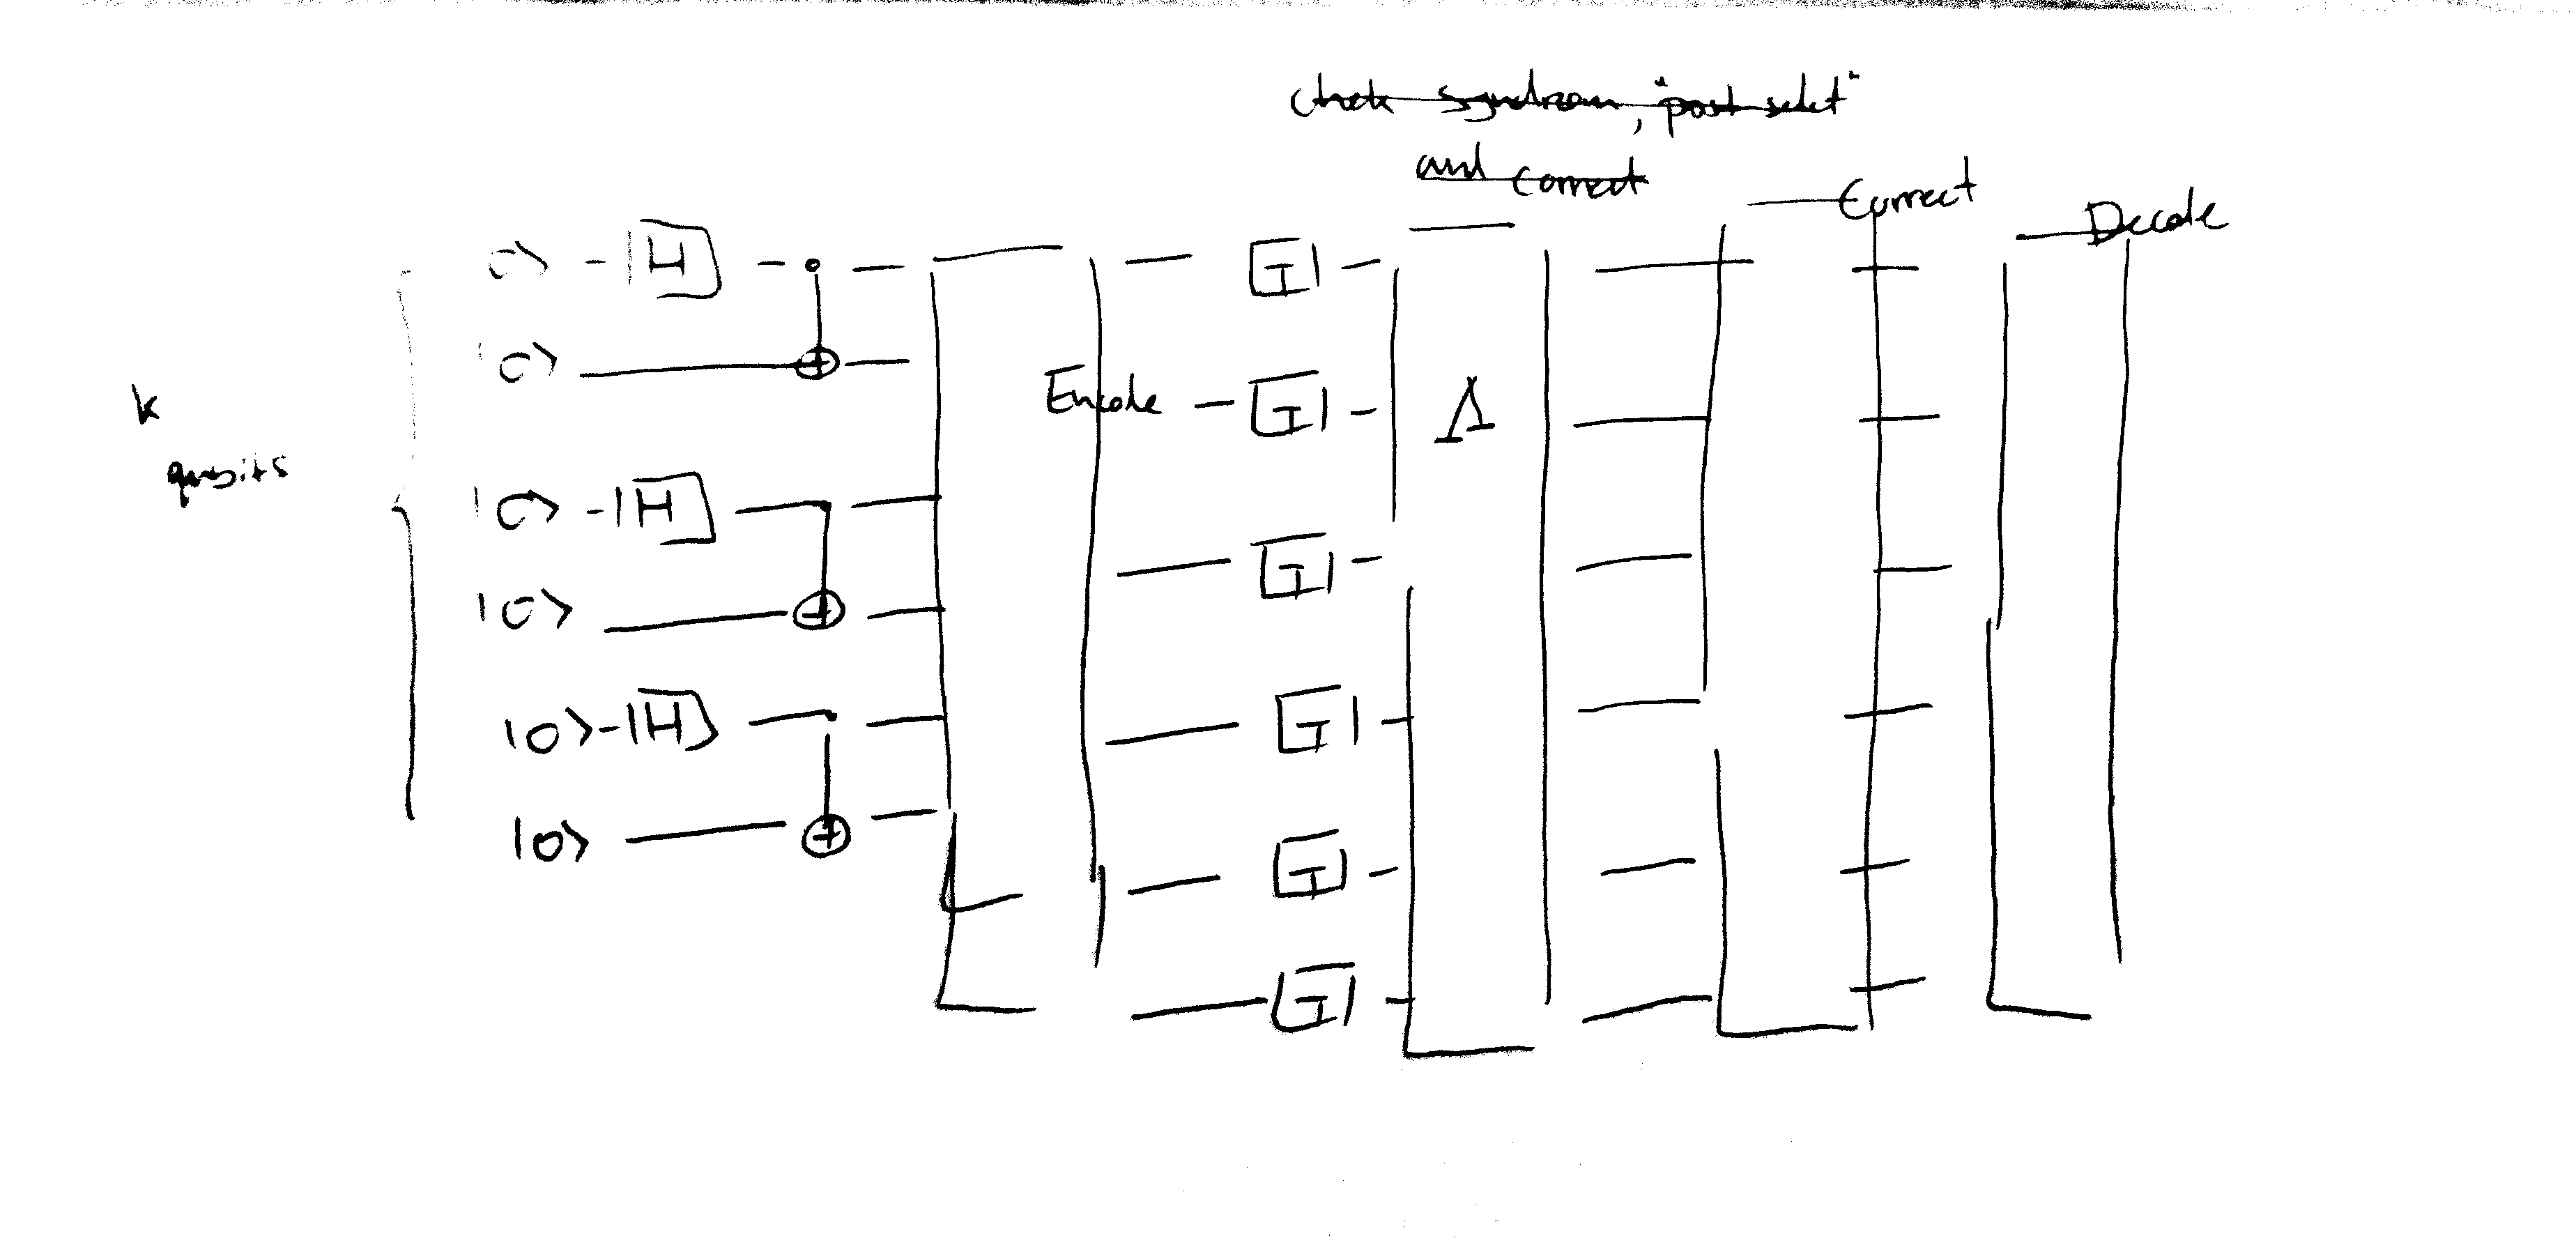
\includegraphics{distil.jpg-out.png}
%}
%  \caption{Quantum Circuit for distillation.}
%  \label{fig:circuit}
%\end{figure}
%
%\begin{claim}
%  \label{claim:phase}
%  The gate $\ket{f} \mapsto \exp \Big(  -  i\pi \sum_{g,h \in G/a} X_{g}X_{h}|g\cdot h|  \Big) \ket{f} $ is in the Clifford.  
%\end{claim}
%\begin{proof}
%Just decode $f$ and apply \textbf{CZ} between any pair of qubits corresponding to the generators $g,h$ such that $g \cap h = 1$. Then encode the state again. Observes that \textbf{CZ} is a Clifford gate, and by the fact that the code is a CSS code then the decoder and the encoder are both in the Clifford.
%\end{proof}
%Let's denote the circuit defined in \Cref{claim:phase} by $\Lambda$. So we have that:  
%\begin{equation*}
%  \begin{split}
%    \Lambda^{\dagger}\exp \Big( i\pi/4 \sum_{g} X_{g}|g|  & -  i\pi \sum_{g,h \in G/a} X_{g}X_{h}|g\cdot h|  \Big) \ket{f} \\
%= & \exp \Big( i\pi/4 \sum_{g} X_{g}|g|  \Big) \ket{f} 
%  \end{split}
%\end{equation*}
%
%Maybe what do we need is to arrange in some way $|g|+|g^{\prime}| = 4k+1$ and $\braket{g,f}= \braket{g^{\prime},f^{\prime}}$
%
%
%\begin{claim}
%  For any $m$ codewords $x_{1}..x_{m}$ there is a set of coordinates $I$ and $|I| < \alpha n$. Such that:  
%  \begin{equation*}
%    \begin{split}
%      \sum_{j \in [n]/I }x_{a}^{j}x_{b}^{j} = 0
%    \end{split}
%  \end{equation*}
%  For any pair $x_{a},x_{b}$. 
%\end{claim}
%
%\begin{claim}
%  For any $m$ codewords $x_{1}..x_{m}$ there is a set of coordinates $I$ and $|I| < \alpha n$. Such that:  
%  \begin{equation*}
%    \begin{split}
%      \sum_{a,b,j \in [n]/I }x_{a}^{j}x_{b}^{j} = 4k
%    \end{split}
%  \end{equation*}
%  For any pair $x_{a},x_{b}$. 
%\end{claim}
%









%\paragraph{What about concatination?} So, take a quantum good code. And consider a prasintion $k^{\prime}|k|m$ such that $k^{\prime} = \dim C_{Z}^{\perp}$ and $k = \dim C_{X}/C_{Z}^{\perp}$. Now concatinate with two genorthogonal codes, such that any logical bit of $k$ has wight of 1 module 8 and the others has weight 0.  



\begin{claim}
  Let $C_{A}$ and $C_{A^\prime}$ such that $C_{A^\prime} \subset C_{A}$. Then $\left(C_{A}^{\perp} \otimes C_{B}^{\perp}  \right)^{\perp}$, $ C_{A^{\prime}} \otimes C_{B^{\prime}}$ form a \textbf{CSS} code $C$ such there exists a subspace $V \subset C$ with effictive distance $d$. 
\end{claim}

\begin{proof}
  Idea. consider generators of the form $e_{0}\otimes g$. Any codeword  in their span is just a first row asssitmentd to a code word of $C_{A}$. If we assume less than linear number on that row then we will secucess to decode it, $+$ some other generators that we don't care about.   
\end{proof}



\begin{equation*}
  \begin{split}
    C_{X} & = \left( \left( C_{A} \otimes C_{0} \right)^{\perp} \otimes C_{0}^{\perp}  \right)^{\perp} \\ 
    C_{Z} & = \left( \left( C_{A} \otimes C_{0} \right) \otimes C_{0}  \right)^{\perp}
  \end{split}
\end{equation*}



\begin{claim}
  \label{claim:oneg}
  Let $C$ be a code at rate $\rho(C) > 7/8 $ has at least one codeword $x \in C$ , such that $|x| =_{8} 1 $.
\end{claim}

\begin{definition}
  We will say that a code $C$ is $(l,m)$-genorthogonal if there exists a generator set $G$ for $C$ such that for any $I \subset G$ such that $1 < |I| < l$ we have that:
  \begin{equation*}
    \begin{split}
      \sum_{i \in [n]}\prod_{g_{j}\in I \subset G}g_{j}^{i} =_{m} 0 
    \end{split}
  \end{equation*}
\end{definition}

\begin{claim} \label{claim:goodgen} 
  If there exists a single $(l,m)$-genorthogonal code for a finite length $\Delta$, then there is a family of $(l,m)$-genorthogonal good codes. Moreover, if there exists a generator in $C_0$ of weight $|\cdot|_m = 1$, then there exists a family that also has at least one generator of weight $|\cdot|_m = 1$.
\end{claim}
\begin{proof}
  Denote by $C_{0} = \Delta[1,\rho_{0}, \delta_{0}]$ an $(l,m)$-genorthogonal code and observes that for any $C = [n,\rho n, \delta n]$ the tensor code $C_{0}\otimes C = [\Delta n, \rho_{0} \rho \Delta n, \delta_{0} \delta \Delta n]$ is also $(l,m)$-genorthogonal code. 

  For the seconed part of the claim, Choose $C$ to be a good code with rate $> \left(2^{m}-1\right)/2^{m}$ by \Cref{claim:oneg} there is at least on codeword $c$ in $C$ such that $|c| =_{m} 1$.

  So pick the base for $C_{0}\otimes C$ such the first generator is $g_{0} \otimes c$ where $g_{0}$ denote a generator of $C_{0}$ satisfies $|g_{0}| =_{m} 1$. 
    Then $|g_{0} \otimes c | = |g_{0}| \cdot |c| =_{m} 1$.  
\end{proof}

\begin{claim}
  Suppose that there exists $(m+1,m)$-genorthogonal code, such that any generator of it has weight $| \cdot | =_{m} 1$ then there exists also a family of good $(m+1,m)$-genorthogonal codes such that a liner portion of his generators $g$ have weight $|g| =_{m} 1$. 
\end{claim}

\begin{proof}  
  Denote by $C_{0}$ a finte $(m+1,m)$-genorthogonal code, such that any generator of it has weight $| \cdot | =_{m} 1$. Let $C$ be a good $(m+1,m)$-genorthogonal code with generator $c$ such that $|c| =_{m} 1$, the existence of which is given by \Cref{claim:goodgen}. Denote its rate by $\rho$. If $C$ has more than $\rho/m \cdot n$ generators at weight $| \cdot | =_{m} 1$ then we are done. Otherwise, by the pigeonhole principle, there is an $i$ such that more than $\rho/m$ portion of the generators are at weight $ |\cdot| =_{m} i$. Denote them by $g_{1},g_{2},g_{3}, \dots, g_{m}$.

  Define the set $g_{1}^{^\prime},g_{2}^{\prime}..g_{m}^{\prime}$ as   
  \begin{equation*}
    \begin{split}
      g^{\prime}_{t} & = c + \sum_{j=t}^{t+m}g_{j} \\
      & \Rightarrow |g^{\prime}_{t+1}| = |c| + \sum_{t}{ |g_{j}| } + \sum_{|I|<l+1}\left|\prod_{g \in I  } \alpha_{\star} g \right| \\
      & =_{m} c + m\cdot i =_{m} c =_{m} 1  
    \end{split}
  \end{equation*}  
Now take $C_0 \otimes C$, and set the new generator set to be $g^0_i \otimes g'_j$. And it's easy to verify that we got the code we wanted.
\end{proof}

\begin{claim} \label{claim:code}
  There exists, a good LDPC code (classic) $C$ such that $C^{\perp}$ is also a good code and a generator set $G$, for exists $G^{\prime} \subset G$ and $|G^{\prime}| = \Theta( |G|)$ such:  
  \begin{enumerate}
    \item For any pair $x \neq y \in G^{\prime} \rightarrow x\cdot y =_{8} 0$
    \item For any triple $x\neq y,z \in G^{\prime} \rightarrow \sum_{i}x_{i}y_{i}z_{i} =_{8} 0$
    \item For any $x \in G^{\prime} \rightarrow |x| =_{8} 1$  
  \end{enumerate}
\end{claim}


\begin{claim}  
  There is $n \rightarrow \Theta(n)$ magic states distillation into a binary qldpc code with $\Theta(\sqrt{n})$ distance, and therefore with asymptotic overhead approaching $1$ 
\end{claim}

\begin{proof}
For the encoding we are going to use the hyperproduct code defined in \cite{Tillich_2014}. Let $C$ be the code given by \Cref{claim:code} and consider the hyperproduct of $C$ with itself $Q = Q(C \times_{H} C)$. In addition, denote by $C_{X},C_{Z}$ the CSS representation of $Q$. 

By the fact that $C^\perp$ is also a good code, then $Q$ is a positive rate, square root distance code. Let $\rho$ be the rate of $C$ and $1 - \rho$ be the rate of $C^{\perp}$. As $\rho > 0$, then one can find $I \subset [n]$ coordinates such that for any $i \in I$ the indicator $e_{i} \not\in C^{\perp}$. Hence, it holds from \cite{Tillich_2014} that any vector of the form $e_{i}\otimes x$ is a codeword of $C_{X}/C_{Z}^{\perp}$.

Denote by $\rho^{\prime}$ the portion of $G^{\prime}$ as defined in \Cref{claim:code}, and define $S$ to be: 
\begin{equation*}
  \begin{split}
    S = \left\{ e_{i} \otimes x| e_{i} \not\in C^{\perp}, x \in G^{\prime} \right\}
  \end{split}
\end{equation*}
Observes that $|S| = \rho^{\prime}\rho n^{2}$ and in addition $S$ satisfies the properties in \Cref{claim:code}. Denote by $f$ a codeword supported only on $S$ and denote by $X_{s}$ the indecator that indicate that $s$ supports $f$. Thus:  
\begin{equation*}
  \begin{split}
    T^{\otimes n}\ket{f}  = \exp \Big( i\pi/4 & \sum_{g} X_{g} \overbrace{|g|}^{8k+1}  \\ 
    & -  2 \cdot i \pi/4  \overbrace{\sum_{g,h} X_{g}X_{h}|g\cdot h|}^{8k} \\ 
  & +  4 \cdot i\pi/4 \overbrace{ \sum_{g,h} X_{g}X_{h}X_{l}|g\cdot h \cdot l| }^{8k } \Big) \ket{f} \\
  & \\ 
  =   \exp \Big( i\pi/4 & \sum_{g \in S} X_{g} \Big) \ket{f}
      \end{split}
\end{equation*}
Therefore we can, generate the enocded (\ctt{For now without spanning on on $C_{Z }^{\perp}$} ) product of $T^{\otimes|S|}\ket{+}^{|S|}$:
\begin{equation*}
  \begin{split}
    \prod_{s \in S} \Big( \ket{0} + \exp \left( i\pi/4 \right) \ket{s} \Big)
  \end{split}
\end{equation*}

\ctt{What is left: 
  \begin{enumerate}
    \item Show that one can generate $ \prod_{s \in S} \Big( \ket{C_{Z}^{\perp}} + \exp \left( i\pi/4 \right) \ket{C_{Z}^{\perp} + s} \Big)$ without propagate the errors. I think I know how to do it.
    \item Compute a threshold $p_{0}$ for using Baravi construction.
  \end{enumerate}
}

Thus we have that $\gamma = \log(n/k)/\log(d) =  \log(n/|S|)/\log(\Theta(\sqrt{n})) \rightarrow 0$ and the overhead growes as $\log^{\gamma}(n) \rightarrow 1$ \cite{bravyi2012magic}, \cite{meier2012magicstate}.
\end{proof}

% Triorthogonal



\printbibliography
\end{document}






My responsibility spreads across the entire pipeline, including implementing features on the chip (cpp, 'realtime') and supporting the map synthesis on the cloud (python).
